\documentclass{article}
\usepackage[utf8]{inputenc}
\usepackage[margin=1 in]{geometry}
\usepackage{graphicx}
\usepackage[colorlinks]{hyperref}
\usepackage{listings}
\usepackage{color}
\usepackage{algorithm}
\usepackage{algorithmic}
\usepackage{float} 

\hypersetup{
  colorlinks=true,
  urlcolor=blue
}

\definecolor{dkgreen}{rgb}{0,0.6,0}
\definecolor{gray}{rgb}{0.5,0.5,0.5}
\definecolor{mauve}{rgb}{0.58,0,0.82}

\lstset{frame=tb,
  language=Python,
  aboveskip=3mm,
  belowskip=3mm,
  showstringspaces=false,
  columns=flexible,
  basicstyle={\small\ttfamily},
  numbers=left,
  numberstyle=\tiny\color{gray},
  keywordstyle=\color{blue},
  commentstyle=\color{dkgreen},
  stringstyle=\color{mauve},
  breaklines=true,
  breakatwhitespace=true,
  tabsize=3
}


\author{Matheus Augusto da Silva - Alessandro Montaldo}
\title{\textbf{SR2I 203 - État de l'art, études initiaux}}
\date{\today}

\begin{document}
\maketitle
%--------------------------
\section{Introduction}
Notre projet s'agit de réaliser un étude et une implémentation d'un type spécifique d'attaque DoS; il s'agit d'un attaque Low and Slow, plus spécifiquement,
l'attaque slowloris. L'objectif de ce rapport est d'introduire les études et progrès faites, ainsi comme expliquer et motives nos prochains pas.
Notamment on a suivi le chemin à la suite:

\begin{itemize}
	\item un étude avec la priorité de comprendre la fonctionnalité principal du protocole HTTP et d'un serveur Web
	\item une recherche capable de bien comprendre le fonctionnement du attaque slowloris
	\item réaliser une implémentation d'un petit programme capable d'envoyer requêtes GET
\end{itemize}

%--------------------------
\section{Étude du Protocole HTTP}
Hypertext Transfer Protocol a été conçu avec le but de construire une architecture client-serveur tel que l'on peut implémenter un déploiement du WWW. C'est un protocole de la couche application et il permet l'implémentation d'un des outils les plus populaires d'Internet aujourd'hui: le navigateur Web.
Le principe c'est d'une architecture où un site web (serveur ou ensemble de serveurs) est associé à plusieurs ressources lesquelles un client peut demander via les méthodes HTTP. Un serveur web peut être identifié par son URL ou son adresse IP et généralement garde informations comme pages web, images et fichiers.

\subsection{HTTP Requests and responses}
Each request begins with a Request-Line that indicates specific method, the resource to which the method applies, and the version of http that the client can support. One or more message headers can follow and a message body separated with a blank line. \\

\noindent
Réponses HTTP sont très similaires à requêtes HTTP.La seule différence significative est que réponses commencent avec un \textit{status line} lorsque
requêtes ont pour début une \textit{request line}.

\begin{figure}[H]
	\begin{center}
		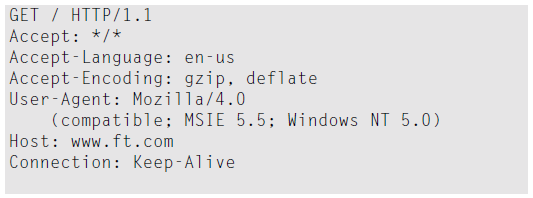
\includegraphics[width=0.6\textwidth]{images/getRequest.png} % Include the image placeholder.png
		\caption{Exemple de GET request.}
                \label{get-request}
	\end{center}
\end{figure}

%--------------------------
\section{Étude du Serveur Web Apache}
Apache est le serveur Web le plus populaire sur Internet. Plus que la majorité des sites Web sont basés sur lui. Ce qui rend Apache vulnérable à l'attaque qui sera analysé, c'est la manière dont il traite ses clients. En particulier, après avoir reçu une requête HTTP, un nouveau fil associé à cette conversation s'ouvrira. \\
Les serveurs Apache plus anciens utilisent un modèle de limitation de thread, généralement un serveur Apache normal peut ouvrir environ 200 threads en parallèle. Normalement, la limitation n’est pas un problème pour les serveurs de site de petite taille, dans la mesure où ils n’ont pas besoin de gérer leur trafic.

\subsection{Nginx vs Apache}
Nginx a été créé pour résoudre le problème de la gestion d’un grand nombre de connexions. Enfait, au lieu d’une architecture à base de threads, comme Apache, Nginx a une architecture pilotée par les événements qui ne crée pas de nouveau processus pour chaque requête. Dans notre projet, nous testerons l’attaque de slowloris sur différents serveurs Web et verrons si l’expérimentation réussira. Dans les cas de serveurs plus résilients, on essayera de faire une version distribuée du attaque, ce qui nous permettra d'attaquer sites plus résilients.

%--------------------------
\section{Étude du attaque Slowloris}
L'idée de base de l'attaque de slowloris est d'ouvrir de nombreuses connexions en envoyant des requêtes HTTP partielles. Des fractions de la demande sont envoyées ultérieurement à intervalles réguliers pour empêcher les sockets de se fermer.
On peut diviser un exploit suivant l'algorithme suivant:

\begin{itemize}
	\item On crée une requête GET destinée au serveur cible
	\item On envoie la requête très lentement et d'une façon incomplète
	\item On répète la même procédure avec un numero très grand de messages, entre 100 et 200, dépendant des configurations du serveur.
	\item Chaque GET répondu sera interprète dans le serveur comme un nouveau client; ça ouvre un nouveau thread dans le réservoir limité du serveur.
	\item Avec le temps, les requêtes lentes mais continues de la machine attaquante iront remplacer tous les connexions "légitimes".
\end{itemize}

\subsection{Slowloris detectability}
A desireble property of an attack is its detectability. After the slowloris attack starts any attached on the log file won't be done until the requests are completed. Once the request is completely sent or once the session gets shut down there will be a log trace of the connection, this means that several hundred 400 errors in the web server logs will be presents,  although it may be possible to turn them into 200 OK messages instead by completing a valid request.

%--------------------------
\section{Implémentation en Python}
\subsection{Programmation}
Le travail d'implémentation a commencé en déterminant les aspects principaux requises. Fonctionnellement, nous avions
besoin d'un petit programme capable d’envoyer requêtes HTTP.Comme nous disons la section d'avant,
l'attaque \textit{slowloris} est fonctionnellement très élégant; en exploitant le mécanisme des GET
requests du protocole HTTP plusieurs fois, on occupe tous les \textit{threads} disponibles au serveur.
Alors, comme le but de notre état de l'art, on a fixé l'objectif d’implémenter un programme capable d'envoyer
GET requests à un serveur web HTTP.Cette fonctionnalité pourra après être déléguée à une fonction en python,
que l'on appellera lors de l'attaque dans une structure de contrôle plus intelligente.
Le but est d'utiliser les méthodes de Scapy, ce qui nous donnera la capacité de contrôler d'une façon plus granulaire
l'envoie des paquets. Le code source est travaillé et managé à travers de
git et le dépôt est disponible publiquement sur Github (documenté en anglais) sur le lien \href{https://github.com/AlessandroMontaldo/slowLorisAttack}{https://github.com/AlessandroMontaldo/slowLorisAttack}

\begin{lstlisting}
#!/usr/bin/env python
# Imports
from scapy.all import *
#import scapy_http.http

# TITLE: http.py
# AUTHORS: Matheus Augusto da Silva; Alessandro Montaldo
# OBS: The following command stops Linux machines from dropping
# the packets generated by scapy (run as root):
# iptables -A OUTPUT -p tcp --tcp-flags RST RST -j DROP

# The goal is to send a well-formated GET request, and not to wait
# for a reponse (200 OK) from the server.
# For the next part of the project, this will be restructured into a function
# which receives and IP address & port number and returns the HTTP response to the GET

# This handles HTTP responses from the server, will be correctly implemented later
# (we're actually having some package importing problems, but since this functionality
# isn't really needed, we'll keep things simple for now)
#def handle(pkt):
#    if pkt.haslayer(http.HTTPrequest):
#        print(pkt)
    
# Make a TCP SYN
#ip_address="35.204.58.85"    # Alessandro's server
ip_address="192.168.33.10"    # Matheus' VM (see Vagrantfile)
server_port=80                # http port
ip = IP(dst=ip_address)       # IP Packet 

# HTTP GET Request
get = "GET / HTTP/1.1\r\nHost: " + ip_address + "\r\n\r\n"
port = RandNum(1024,6500)

# The TCP 3-way handshake rules must be followed. As such, we begin by sending a
# TCP packet with the S (or SYN) flag set. The sequence number is irrelevant, as all
# future TCP packets will contain sequence numbers which are increments of the number
# given
SYN = ip/TCP(sport=port, dport=server_port, flags="S", seq=42) 

# Send SYN and wait for SYNACK as response
print(SYN.summary())
SYNACK = sr1(SYN)

# Send ACK and finally HTTP GET, sniff for the result
ACK=ip/TCP(sport=SYNACK.dport, dport=server_port, flags="A", seq=SYNACK.ack, ack=(SYNACK.seq+1))/get
send(ACK)
#sniff(filter="tcp and port 80", store=False, prn=handle) # we'll improve on this later 
\end{lstlisting}


\subsection{Résultats}
Le code montré avant est l'état de l'art. Il peut effectivement envoyer les requêtes incomplètes que l'on veut
avec un simple changement de la string ``get''. En l’exécutant avec la commande python2 et en regardant 
le flux de messages sur Wireshark, on voit qu'il a bien réussi d'envoyer messages du type HTTP. Le
\textit{3-way-handshake} du protocole TCP est codé manuellement, faisant attention aux champs de
\textit{ack-number} et \textit{sequence-number}. Le serveur est capable de comprendre les requêtes et
répondre avec une message 200 OK tout en bas.


\begin{figure}[H]
	\begin{center}
          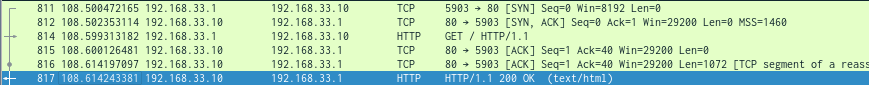
\includegraphics[width=0.8\textwidth]{images/3wayhandshake-get.png} % Include the image placeholder.png
		\caption{Résultats vus sur Wireshark}
                \label{wireshark-dialogue}
	\end{center}
\end{figure}

%--------------------------
\section{Travaux futurs}
Le but des prochains travaux sera d'effectivement mettre une couche logique sur la méthode GET de tel façon
à obtenir le comportement attendu. Dans ce moment, la fonction principal du travail est http.py. La prochaine
étape sera de la transformer en une fonction qui reçoit un adresse IP et un numéro de porte. La logique d'allouer
numéro de portes sera toute faite par loris.py, que l'on développera à la suite.

\begin{thebibliography}{}

\bibitem{rfc}{Internet Engineering Task Force (IETF)\\
\href{https://tools.ietf.org/html/rfc1945}{Request for Comment 1945 - Hypertext Transfer Protocol 1.0}}

\bibitem{http-book}{THOMAS, Stephen \\
HTTP Essentials: Protocols for Secure, Scaleable Web Sites}

\bibitem{apache}{The Apache Group \\
\href{https://httpd.apache.org/docs/2.2/fr/new_features_2_0.html.fr}{Vue d'ensemble des nouvelles fonctionnalités d'Apache 2.0}}

\bibitem{apache-attacked}{Christian Folini, LWN.net group, archivé \\
\href{archive.wikiwix.com/cache/?url=http\%3A\%2F\%2Flwn.net\%2FArticles\%2F338407\%2FA}{Apache attacked by a slowloris}}

\bibitem{hackers}{Ha.ckers group, archivé \\
\href{https://web.archive.org/web/20150426090206/http://ha.ckers.org/slowloris}{Slowloris HTTP DoS}}

\bibitem{repo}{Dépôt Github \\
\href{https://github.com/llaera/slowloris.pl}{slowloris.pl, a perl implementation}}

\end{thebibliography}
\end{document}
